\documentclass[a4paper]{article}
\usepackage[T1]{fontenc}			% \chapter package
\usepackage[english]{babel}
\usepackage[english]{isodate}  		% date format
\usepackage{graphicx}				% manage images
\usepackage{amsfonts}
\usepackage{booktabs}				% high quality tables
\usepackage{amsmath}				% math package
\usepackage{amssymb}				% another math package (e.g. \nexists)
\usepackage{bm}                     % bold math symbols
\usepackage{mathtools}				% emphasize equations
\usepackage{stmaryrd} 				% '\llbracket' and '\rrbracket'
\usepackage{amsthm}					% better theorems
\usepackage{enumitem}				% manage list
\usepackage{pifont}					% nice itemize
\usepackage{cancel}					% cancel math equations
\usepackage{caption}				% custom caption
\usepackage[]{mdframed}				% box text
\usepackage{multirow}				% more lines in a table
\usepackage{textcomp, gensymb}		% degree symbol
\usepackage[x11names]{xcolor}		% RGB color
\usepackage[many]{tcolorbox}		% colorful box
\usepackage{multicol}				% more rows in a table (used for the lists)
\usepackage{listings}
\usepackage{url}
\usepackage{qrcode}
\usepackage{fontawesome5}
\usepackage{ragged2e}
\usepackage{cite}                   % references
\usepackage{imakeidx}               % index
\makeindex[program=makeindex, columns=1,
           title=Index, 
           intoc,
           options={-s index-style.ist}]
\usepackage{fancyhdr}
\usepackage{eurosym}                % Euro symbol package

%\pdfcompresslevel=0
%\pdfobjcompresslevel=0

\definecolor{codegreen}{rgb}{0,0.6,0}
\definecolor{codegray}{rgb}{0.5,0.5,0.5}
\definecolor{codepurple}{rgb}{0.58,0,0.82}
\definecolor{backcolour}{rgb}{0.95,0.95,0.92}
\lstdefinestyle{mystyle}{
    backgroundcolor=\color{backcolour},
    commentstyle=\color{codegreen},
    keywordstyle=\color{magenta},
    numberstyle=\tiny\color{codegray},
    stringstyle=\color{codepurple},
    basicstyle=\ttfamily\footnotesize,
    breakatwhitespace=false,
    breaklines=true,
    captionpos=b,
    keepspaces=true,
    numbers=left,
    numbersep=5pt,
    showspaces=false,
    showstringspaces=false,
    showtabs=false,
    tabsize=2
}
\lstset{style=mystyle}


% thanks Mico: https://tex.stackexchange.com/a/60218/312896
\makeatletter
\renewcommand\paragraph{\@startsection{paragraph}{4}{\z@}%
            {-2.5ex\@plus -1ex \@minus -.25ex}%
            {1.25ex \@plus .25ex}%
            {\normalfont\normalsize\bfseries}}
\makeatother
\setcounter{secnumdepth}{4} % how many sectioning levels to assign numbers to
\setcounter{tocdepth}{4}    % how many sectioning levels to show in ToC


% draw a frame around given text
\newcommand{\framedtext}[1]{%
	\par%
	\noindent\fbox{%
		\parbox{\dimexpr\linewidth-2\fboxsep-2\fboxrule}{#1}%
	}%
}


% table of content links
\usepackage{xcolor}
\usepackage[linkcolor=black, citecolor=blue, urlcolor=cyan]{hyperref} % hypertexnames=false
\hypersetup{
	colorlinks=true
}


\newtheorem{theorem}{\textcolor{Red3}{\underline{Theorem}}}
\renewcommand{\qedsymbol}{QED}
\newcommand{\dquotes}[1]{``#1''}
\newcommand{\longline}{\noindent\rule{\textwidth}{0.4pt}}
\newcommand{\circledtext}[1]{\raisebox{.5pt}{\textcircled{\raisebox{-.9pt}{#1}}}}
\newcommand{\definition}[1]{\textcolor{Red3}{\textbf{#1}}\index{#1}}
\newcommand{\example}[1]{\textcolor{Green4}{\textbf{#1}}}
\newcommand{\highspace}{\vspace{1.2em}\noindent}
\newcommand{\version}{v0.2.0}
\newcommand{\opt}{\mathrm{opt} \:}


\begin{document}
    \newcounter{definition}[section]
    \newcounter{example}[section]
    \newcounter{exercise}[section]
    
    \newtcolorbox[use counter = definition]{definitionbox}[1][]{%
        breakable,
        enhanced,
        colback=red!5!white,
        colframe=red!75!black,
        fonttitle=\bfseries,
        title={Definition \thetcbcounter#1} %
    }

    \newtcolorbox[use counter = exercise]{exercisebox}[1][]{%
        breakable,
        enhanced,
        colback=Red3!5!white,
        colframe=Red3!75!black,
        fonttitle=\bfseries,
        title={Exercise \thetcbcounter#1} %
    }
    
    \newtcolorbox[use counter = example]{examplebox}[1][]{%
        breakable,
        enhanced,
        colback=Green4!5!white,
        colframe=Green4!75!black,
        fonttitle=\bfseries,
        title={Example \thetcbcounter#1} %
    }

    \newtcolorbox[]{deepeningbox}[1][]{%
        breakable,
        enhanced,
        colback=DarkOrange3!5!white,
        colframe=DarkOrange3!75!black,
        fonttitle=\bfseries,
        title={Deepening#1} %
    }

    %%%%%%%%%%%%%%%
    % Notes cover %
    %%%%%%%%%%%%%%%
    \author{260236}
\title{Parallel Computing - Notes - \version}
\date{\printdayoff\today}
\maketitle

    %%%%%%%%%%%
    % Preface %
    %%%%%%%%%%%
	\section*{Preface}

Every theory section in these notes has been taken from the sources:
\begin{itemize}
    \item Course slides.\cite{numerical-linear-algebra-polimi}
\end{itemize}
About:
\begin{itemize}
    \item[\faIcon{github}] \href{https://github.com/PoliMI-HPC-E-notes-projects-AndreVale69/HPC-E-PoliMI-university-notes}{GitHub repository}
    \begin{center}
        \qrcode{https://github.com/PoliMI-HPC-E-notes-projects-AndreVale69/HPC-E-PoliMI-university-notes}
    \end{center}
\end{itemize}
These notes are an unofficial resource and shouldn't replace the course material or any other book on numerical linear algebra. It is not made for commercial purposes. I've made the following notes to help me improve my knowledge and maybe it can be helpful for everyone.

As I have highlighted, a student should choose the teacher's material or a book on the topic. These notes can only be a helpful material.

\highspace

\subsection*{Correlated Projects}

During the Numerical Linear Algebra for HPC course, I was part of a team where we created a project that included two challenges related to the course. See more details in the corresponding repository:
\begin{itemize}
    \item[\faIcon{github}] \href{https://github.com/PoliMI-HPC-E-notes-projects-AndreVale69/NLA-challenges}{GitHub repository}
    \begin{center}
        \qrcode{https://github.com/PoliMI-HPC-E-notes-projects-AndreVale69/NLA-challenges}
    \end{center}
\end{itemize}

    %%%%%%%%%%%%%%%%%%%%%
    % Table of contents %
    %%%%%%%%%%%%%%%%%%%%%
    \tableofcontents
    \newpage

    %%%%%%%%%%%%%%%%
    % Introduction %
    %%%%%%%%%%%%%%%%
    \section{Introduction}

\begin{definitionbox}
    \definition{Operations Research (OR)}, often shortened to the initialism \texttt{OR}, is the branch of mathematics in which \textbf{mathematical models} and \textbf{quantitative methods} (e.g. optimization, game theory, simulation) are \textbf{used to analyze complex decision-making problems} and \textbf{find (near-)optimal solutions}.
\end{definitionbox}

\highspace
The overall and primary \emph{goal} is to \emph{help make better decisions}.

\highspace
OR can be seen as an interdisciplinary field at the intersection of applied mathematics, computer science, economics, and industrial engineering.

\highspace
Operations research is often concerned with \textbf{determining the extreme values of some real-world objective}: the \emph{maximum} (of profit, performance, or yield) or \emph{minimum} (of loss, risk, or cost). Originating in military efforts before World War II, its techniques have grown to concern problems in a variety of industries.\cite{wikipediaOperationsResearch}

\longline

\subsection{Decision-making problems}

Decision-making problems are analyzed using mathematical models and quantitative methods.

\begin{definitionbox}
    \definition{Decision-making problems} are problems in which we must \textbf{choose} a (feasible) \textbf{solution among a large number of alternatives based on one or several criteria}.
\end{definitionbox}

\highspace
Some practical \example{examples} include network design, shortest paths, staff scheduling, and service management.

\highspace
In other words, they are complex decision-making problems that are \textbf{addressed through a mathematical modeling approach} (mathematical models, algorithms, and computer implementations).
    \subsection{Scheme of an OR study}

The most important and common \textbf{steps} in operational research are:
\begin{enumerate}
    \item \textbf{Problem}. Define the problem;
    \item \textbf{Model}. Build the model;
    \item \textbf{Algorithm}. Select or develop an appropriate algorithm;
    \item \textbf{Implementation}. Implementing or using an efficient computer program;
    \item \textbf{Results}. Analyze the results.
\end{enumerate}

\begin{definitionbox}
    A mathematical \definition{model} is a \textbf{simplified representation of a real-world problem}.
\end{definitionbox}

\noindent
To define a mathematical model, it is necessary to identify the fundamental elements of the problem and the main relationships between them. But \textbf{how can we decide} the \emph{number of decision makers}, the \emph{number of objectives} and the \emph{level of uncertainty in the parameters}? It depends on the environment. If we have:
\begin{itemize}
    \item One decision maker, one object, then we will use \textbf{mathematical programming}.
    \item One decision maker, multiple objectives, then we will use \textbf{multi-objective programming}.
    \item Uncertainty greater than zero, then we will use \textbf{stochastic programming}.
    \item Multiple decision makers, then we will use \textbf{game theory}.
\end{itemize}

\highspace
\begin{examplebox}[: production planning]
    A company produces 3 types of electronic devices: $D_{1}$, $D_{2}$, $D_{3}$; going through 3 main phases of the production process: assembly, refinement and quality control.

    Time (in minutes) required for each phase and product:

    \begin{center}
        \begin{tabular}{@{} c | c c c @{}}
            & $D_{1}$ & $D_{2}$ & $D_{3}$ \\
            \midrule
            Assembly        & $80$ & $70$ & $120$ \\
            Refinement      & $70$ & $90$ & $20$ \\
            Quality control & $40$ & $30$ & $20$
        \end{tabular}
    \end{center}

    Available resources within the planning horizon (depend on the workforce) in minutes:
    \begin{center}
        \begin{tabular}{@{} c | c | c @{}}
            Assembly & Refinement & Quality control \\
            \midrule
            $30'000$ & $25'000$ & $18'000$
        \end{tabular}
    \end{center}

    Unitary profit (in KEuro):
    \begin{center}
        \begin{tabular}{@{} c | c | c @{}}
            $D_{1}$ & $D_{2}$ & $D_{3}$ \\
            \midrule
            $1.6$ & $1$ & $2$
        \end{tabular}
    \end{center}
    
    Assumption: the company can sell whatever it produces.

    \emph{Give a mathematical model for determining a production plan which maximizes the total profit.}

    \begin{itemize}
        \item \textbf{Decision variables}, $x_{j}$ is equal to the number of devices $D_{j}$ produced, for $j = 1, 2, 3$.
        
        \item \textbf{Objective function}: $\max \: z = 1.6x_{1} + 1x_{2} + 2x_{3}$.

        \item \textbf{Constraints}: the production capacity limit for each phase:
        \begin{equation*}
            \begin{array}{rcl}
                80x_{1} + 70x_{2} + 120x_{3} &\le& 30'000 \hspace{2em} \text{(assembly)} \\ [.5em]
                70x_{1} + 90x_{2} + 20x_{3} &\le& 25'000 \hspace{2em} \text{(refinement)} \\ [.5em]
                40x_{1} + 30x_{2} + 20x_{3} &\le& 18'000 \hspace{2em} \text{(quality control)}
            \end{array}
        \end{equation*}

        \item \textbf{Non-negative variables}: $x_{1}, x_{2}, x_{3} \ge 0$ may be fractional (real) values.
    \end{itemize}
\end{examplebox}

\begin{examplebox}[: portfolio selection problem]
    An insurance company must decide which investments to select out of a given set of possible assets (stocks, bonds, options, gold certificates, real estate, \dots).

    \begin{center}
        \begin{tabular}{@{} c | c c c @{}}
            Investments & area & capital $\left(c_{j} \: K€\right)$ & expected return $\left(r_{j}\right)$ \\
            \midrule
            A & Germany & $150$ & $11\%$ \\
            B & Italy & $150$ & $9\%$ \\
            C & U.S.A. & $60$ & $13\%$ \\
            D & Italy & $100$ & $10\%$ \\
            E & Italy & $125$ & $8\%$ \\
            F & France & $100$ & $7\%$ \\
            G & Italy & $50$ & $3\%$ \\
            H & UK & $80$ & $5\%$
        \end{tabular}
    \end{center}
    Legend:
    \begin{itemize}
        \item A and B: automotive
        \item C and D: ICT
        \item E and F: real estate
        \item G: short term treasury bounds
        \item H: long term treasury bounds
    \end{itemize}
    The available capital is: $600$ KEuro.

    At most 5 investments to avoid excessive fragmentation.

    Geographic diversification to limit risk: $\le 3$ investments in Italy and $\le 3$ abroad.

    \emph{Give a mathematical model for deciding which investments to select so as to maximize the expected return while satisfying the constraints.}

    \begin{itemize}
        \item \textbf{Decision variables}, $x_{j}$ is equal to $1$ if $j$-th investment is selected and $x_{j}=0$ otherwise, for $j = 1, \dots, 8$.
        
        \item \textbf{Objective function}: $\max \: z = \displaystyle\sum_{j=1}^{8} c_{j} \: r_{j} \: x_{j}$.

        \item \textbf{Constraints}:
        \begin{equation*}
            \begin{array}{rclcl}
                \displaystyle\sum_{j=1}^{8}c_{j} \: x_{j} &\le& 600 &\hspace{1em}& \text{(capital)} \\ [2em]
                \displaystyle\sum_{j=1}^{8}x_{j} &\le& 5 &\hspace{1em}& \text{(max 5 investments)} \\ [2em]
                x_{2}+x_{4}+x_{5}+x_{7} &\le& 3 &\hspace{1em}& \text{(max 3 in Italy)} \\ [.5em]
                x_{1}+x_{3}+x_{6}+x_{8} &\le& 3 &\hspace{1em}& \text{(max 3 abroad)}
            \end{array}
        \end{equation*}

        \item \textbf{Binary (integer) variables}: $x_{j} \in \left\{0,1\right\}$ and $1 \le j \le 8$.
    \end{itemize}

    \underline{\textbf{Possible variant}}. In order to limit the risk, if any of the ICT investment is selected then at least one of the treasury bond must be selected.
    \begin{itemize}
        \item \textbf{Objective function}: $\max z = \displaystyle\sum_{j=1}^{8} c_{j} \: r_{j} \: x_{j}$.

        \item \textbf{Constraints}:
        \begin{equation*}
            \begin{array}{rcll}
                \displaystyle\sum_{j=1}^{8}c_{j} \: x_{j} &\le& 600 & \text{(capital)} \\ [2em]
                \displaystyle\sum_{j=1}^{8}x_{j} &\le& 5 & \text{(max 5 investments)} \\ [2em]
                x_{2}+x_{4}+x_{5}+x_{7} &\le& 3 & \text{(max 3 in Italy)} \\ [.5em]
                x_{1}+x_{3}+x_{6}+x_{8} &\le& 3 & \text{(max 3 abroad)} \\ [1em]
                \dfrac{x_{3} + x_{4}}{2} &\le& x_{7} + x_{8} & \text{(investment in treasury bonds)}
            \end{array}
        \end{equation*}

        \item \textbf{Binary (integer) variables}: $x_{j} \in \left\{0,1\right\}$ and $1 \le j \le 8$.
    \end{itemize}
\end{examplebox}

\newpage

\begin{examplebox}[: facility location]
    Consider 3 oil pits, located in positions $A$, $B$ and $C$, from which oil is extracted.

    \begin{center}
        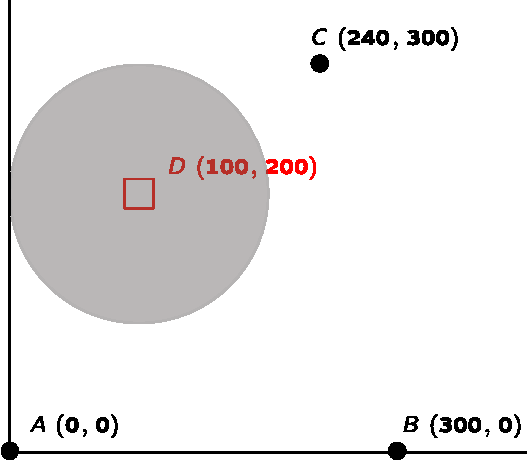
\includegraphics[width=.6\textwidth]{img/facility-location-1.pdf}
    \end{center}

    Connect them to a refinery with pipelines whose cost is proportional to the square of their length.

    The refinery must be at least 100 km away from point $D = \left(100, 200\right)$, but the oil pipelines can cross the corresponding forbidden zone.

    \emph{Give a mathematical model to decide where to locate the refinery so as to minimize the total pipeline cost.}

    \begin{itemize}
        \item \textbf{Decision variables}, $x_{1}, x_{2}$ cartesian coordinates of the refinery.
        
        \item \textbf{Objective function}:
        \begin{equation*}
            \begin{array}{rl}
                \min z = & \left[\left(x_{1} - 0\right)^{2} + \left(x_{2} - 0\right)^{2}\right] + \\ [.5em]
                         & \left[\left(x_{1} - 300\right)^{2} + \left(x_{2} - 0\right)^{2}\right] + \\ [.5em]
                         & \left[\left(x_{1} - 240\right)^{2} + \left(x_{2} - 300\right)^{2}\right]
            \end{array}
        \end{equation*}

        \item \textbf{Constraints}:
        \begin{equation*}
            \sqrt{
                \left(x_{1}-100\right)^{2} + \left(x_{2} - 200\right)^{2}
            } \ge 100
        \end{equation*}

        \item \textbf{Variables}: $x_{1}, x_{2} \in \mathbb{R}$.
    \end{itemize}
\end{examplebox}
    \subsection{Mathematical programming/optimization}

\definition{Mathematical Optimization} or \definition{Mathematical Programming} is the \textbf{selection of a best element}, with regard to some criteria, \textbf{from some set of available alternatives}.

In the more general approach, an optimization problem consists of \textbf{maximizing} or \textbf{minimizing a real function} by systematically choosing input values from within an allowed set and computing the value of the function. The generalization of optimization theory and techniques to other formulations constitutes a large area of applied mathematics.

\highspace
\begin{flushleft}
    \textcolor{Green3}{\faIcon{question-circle} \textbf{And where should we start?}}
\end{flushleft}
Decision-making problems are characterized by a \textbf{single decision maker}, a \textbf{single objective}, and \textbf{reliable parameter estimates}. Using mathematical language, we can say:
\begin{equation*}
    \opt f\left(\mathbf{x}\right) \hspace{1em} \text{with} \hspace{1em} \mathbf{x} \in X \hspace{1em} \text{and} \hspace{1em} \opt = \begin{Bmatrix}
        \min \\ \max
    \end{Bmatrix}
\end{equation*}
Where:
\begin{itemize}
    \item $\mathbf{x} \in \mathbb{R}^{n}$ \textbf{decision variables}. They are numerical variables whose values identify a solution of the problem.

    \item $X \subseteq \mathbb{R}^{n}$ \textbf{feasible region}. Distinguishes between feasible and infeasible solutions (via constraints):
    \begin{equation*}
        X = \left\{\mathbf{x} \in \mathbb{R}^{n} \: : \: g_{i}\left(\mathbf{x}\right) \begin{Bmatrix}
        = \\ \le \\ \ge
        \end{Bmatrix} 0, i = 1, \dots, m\right\}
    \end{equation*}

    \item $f: X \rightarrow \mathbb{R}$ \textbf{objective function}.Expresses in quantitative terms the value or cost of each feasible solution.
\end{itemize}
Note an interesting observation:
\begin{equation*}
    \max\left\{f\left(\mathbf{x}\right): \: \mathbf{x} \in X\right\} = -\min\left\{-f\left(\mathbf{x}\right): \: \mathbf{x} \in X\right\}
\end{equation*} 
    \subsection{Multi-objective programming}\label{subsection: Multi-objective programming}

\begin{flushleft}
    \textcolor{Green3}{\faIcon{question-circle} \textbf{How is it born?}}
\end{flushleft}
Even though some real-word problems can be reduced to a matter of a single objective very often it is hard to define all the aspects in terms of a single objective. Defining multiple objectives often gives a better idea of the task.

\highspace
\definition{Multi-objective programming} (also known as \definition{Multi-objective optimization} or \definition{Pareto optimization}) is an \textbf{area of multiple-criteria decision making} that is concerned with mathematical optimization problems involving \textbf{more than one objective function to be optimized simultaneously}. Multi-objective is a type of vector optimization that has been applied in many fields of science, including engineering, economics and logistics where optimal decisions need to be taken in the presence of trade-offs between two or more conflicting objectives. 

Minimizing cost while maximizing comfort while buying a car, and maximizing performance whilst minimizing fuel consumption and emission of pollutants of a vehicle are \example{examples} of multi-objective optimization problems involving two and three objectives, respectively.\cite{abraham2005evolutionary}

\highspace
Suppose to minimize $f_{1}\left(\mathbf{x}\right)$ and maximize $f_{2}\left(\mathbf{x}\right)$ (e.g. laptop: $f_{1}$ is cost and $f_{2}\left(\mathbf{x}\right)$ is performance):
\begin{enumerate}
    \item Turn it into a \definition{single objective problem} by expressing the two objectives in terms of the same unit (e.g. monetary unit):
    \begin{equation*}
        \min \lambda_{1}f_{1}\left(\mathbf{x}\right) - \lambda_{2}f_{2}\left(\mathbf{x}\right)
    \end{equation*}
    for appropriate scalars $\lambda_{1}$ and $\lambda_{2}$.

    \item Optimize the \definition{primary objective} function and turn the other objective into a constraint:
    \begin{equation*}
        \underset{x \in \tilde{X}}{\max} f_{2}\left(\mathbf{x}\right) \hspace{1em} \text{where} \hspace{1em} \tilde{X} = \left\{\mathbf{x} \in X \: : \: f_{1}\left(\mathbf{x}\right) \le \varepsilon \right\}
    \end{equation*}
    for appropriate constant $\varepsilon$.
\end{enumerate}
This is a simple introduction, the more detailed explanation will be explained in the following pages.
    \subsection{Mathematical Programming or Simulation?}

Mathematical Programming and Simulation involves \textbf{building a model} and \textbf{designing an algorithm}. And the main differences are:
\begin{table}[!htp]
    \centering
    \begin{tabular}{@{} p{15em} | p{15em} @{}}
        \toprule
        \textbf{Mathematical Programming} & \textbf{Simulation} \\
        \midrule
        Problem can be \dquotes{well} formalized. & Problem is difficult to formalize. \\
        \cmidrule{1-2}
        Algorithm yields a(n optimal) solution. & Algorithm simulates the evolution of the real system and allows to evaluate the performance of alternative solutions. \\
        \cmidrule{1-2}
        The results are \dquotes{certain} & The results need to be interpreted. \\
        \cmidrule{1-2}
        Example: assignment. & Example: service counters. \\
        \bottomrule
    \end{tabular}
    \caption{Major differences between Mathematical Programming and Simulation.}
\end{table}

    %%%%%%%%%%%%%%%%%%%
    % Fancy pagestyle %
    %%%%%%%%%%%%%%%%%%%
    \pagestyle{fancy}
    \fancyhead{} % clear all header fields
    \fancyhead[R]{\nouppercase{\leftmark\hfill\rightmark}}

    %%%%%%%%%%%%%%%%%%%%%%%%%%
    % Bibliography and index %
    %%%%%%%%%%%%%%%%%%%%%%%%%%
    \pagestyle{fancy}
\fancyhead{} % clear all header fields
\fancyhead[R]{\nouppercase{\leftmark}}

\bibliography{bibtex}{}
\bibliographystyle{plain}

\newpage

\printindex
\end{document}